\documentclass[a4paper,10pt]{article}

\usepackage[utf8]{inputenc}
\usepackage[T1]{fontenc}
\usepackage{lmodern}
\usepackage{mathtools}
\usepackage{enumitem}

\usepackage{tikz}
\usetikzlibrary{patterns}
\usetikzlibrary{automata,positioning}
\usetikzlibrary{shapes.multipart}
\usetikzlibrary{matrix}

\usepackage[export]{adjustbox}
\usepackage{listings}
\usepackage{color}


\begin{document}
% import from Mr. Huang
                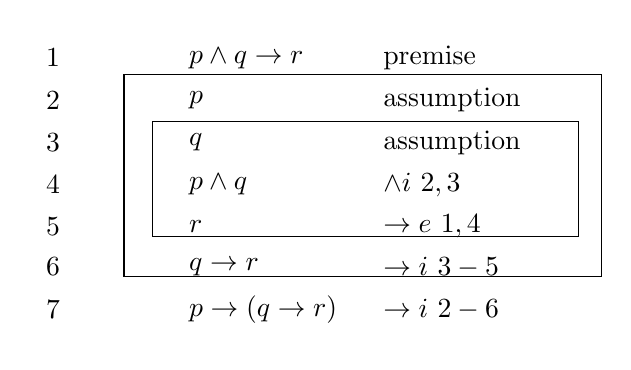
\begin{tikzpicture}[every node/.style={anchor=west}]
                \matrix (m) [matrix of math nodes,
                    nodes in empty cells]{
                    1\quad  \quad & \    & \quad  p\land q \rightarrow r & \quad \textrm{premise} \\
                    2 \quad  \quad & \  & \quad  p   & \quad \textrm{assumption}\\
                    3 \quad  \quad & \  & \quad  q   & \quad \textrm{assumption}\\
                    4 \quad  \quad & \  & \quad  p\land q   & \quad \land i\ 2,3 \\
                    5 \quad  \quad & \  & \quad  r   & \quad \rightarrow e\ 1,4 \\
                    6 \quad  \quad & \  & \quad  q \rightarrow r   & \quad \rightarrow i\ 3-5 \\
                    7 \quad  \quad & \  & \quad  p \rightarrow (q \rightarrow r)   & \quad \rightarrow i\ 2-6 \\
                            };
                            % \pause
                    \draw (m-5-2.south east)  rectangle (7,0.8);
                    \draw (m-6-2.south west)  rectangle (7.3,1.4);
                \end{tikzpicture}
% end of import
\end{document}